%LTeX: language=pt-br
% !TeX root = Apostila_IM381.tex

\section{Introdução}

    \subsection{Sobre a apostila e o método}

        Esta apostila serve como base para a disciplina IM381 - Elementos Finitos I, do programa de Engenharia Mecânica da Faculdade de Engenharia Mecânica da Universidade Estadual de Campinas. Esta apostila tem como objetivo auxiliar os alunos desta disciplina o acompanhamento destes no curso. Ela não tem pretensão de substituir qualquer livro, e um aprendizado adequado aos conteúdos apresentados aqui deve ser feito com auxílio de um bom livro de Elementos Finitos da literatura. 

        Esta apostila se encontra em um estágio inicial ainda, vários erros ainda podem estar presentes nela, entretanto, sugere-se cautela dos alunos estudando com base nela. Em caso de dúvidas, ou caso você deseje reportar algum erro ou fazer alguma sugestão, entre em contato com o autor por \url{hnlopes@unicamp.br}.

    \subsection{Instalação da biblioteca}

        Esta disciplina, quando ministrada pelo autor desta apostila, conta com o auxílio da biblioteca em Python de elementos finitos desenvolvido por seu grupo de pesquisa. Esta biblioteca se chama finelpy (Finite Element Python library). O código base desta biblioteca pode ser encontrado em \url{https://github.com/Lopes941/finelpy}, sendo esta programada nas linguagens Python e C++.

        A instalação dessa biblioteca pode ser feita pelo Python Package Index (PyPI). 

        \begin{center}
            \fbox{pip install finelpy}
        \end{center}

        
        Segue uma breve indicação de como começar a usar o Python em um computador com Windows.

        \subsubsection*{Instalação do Anaconda}

        Anaconda é uma plataforma para distribuição e para rodar programas em linguagem Python. Para alguém que nunca usou essa linguagem, talvez seja a plataforma mais intuitiva para iniciar. A instalação é feita diretamente no site em \url{https://www.anaconda.com/download/success}. Sinta-se livre para baixar a versão completa ou o miniconda.

        Ao instalar, abra o navegador conda (Anaconda Navigator). Na aba ``Home'', haverá vários softwares e IDEs que você pode usar. Aqui, usaremos o Spyder, por se tratar do mais parecido com o MATLAB, com o qual alguns alunos talvez já tenham familiaridade. A página principal do Spyder é conforme a Figura \ref{fig:spyder}.

        \begin{figure}[h!]
            \centering
            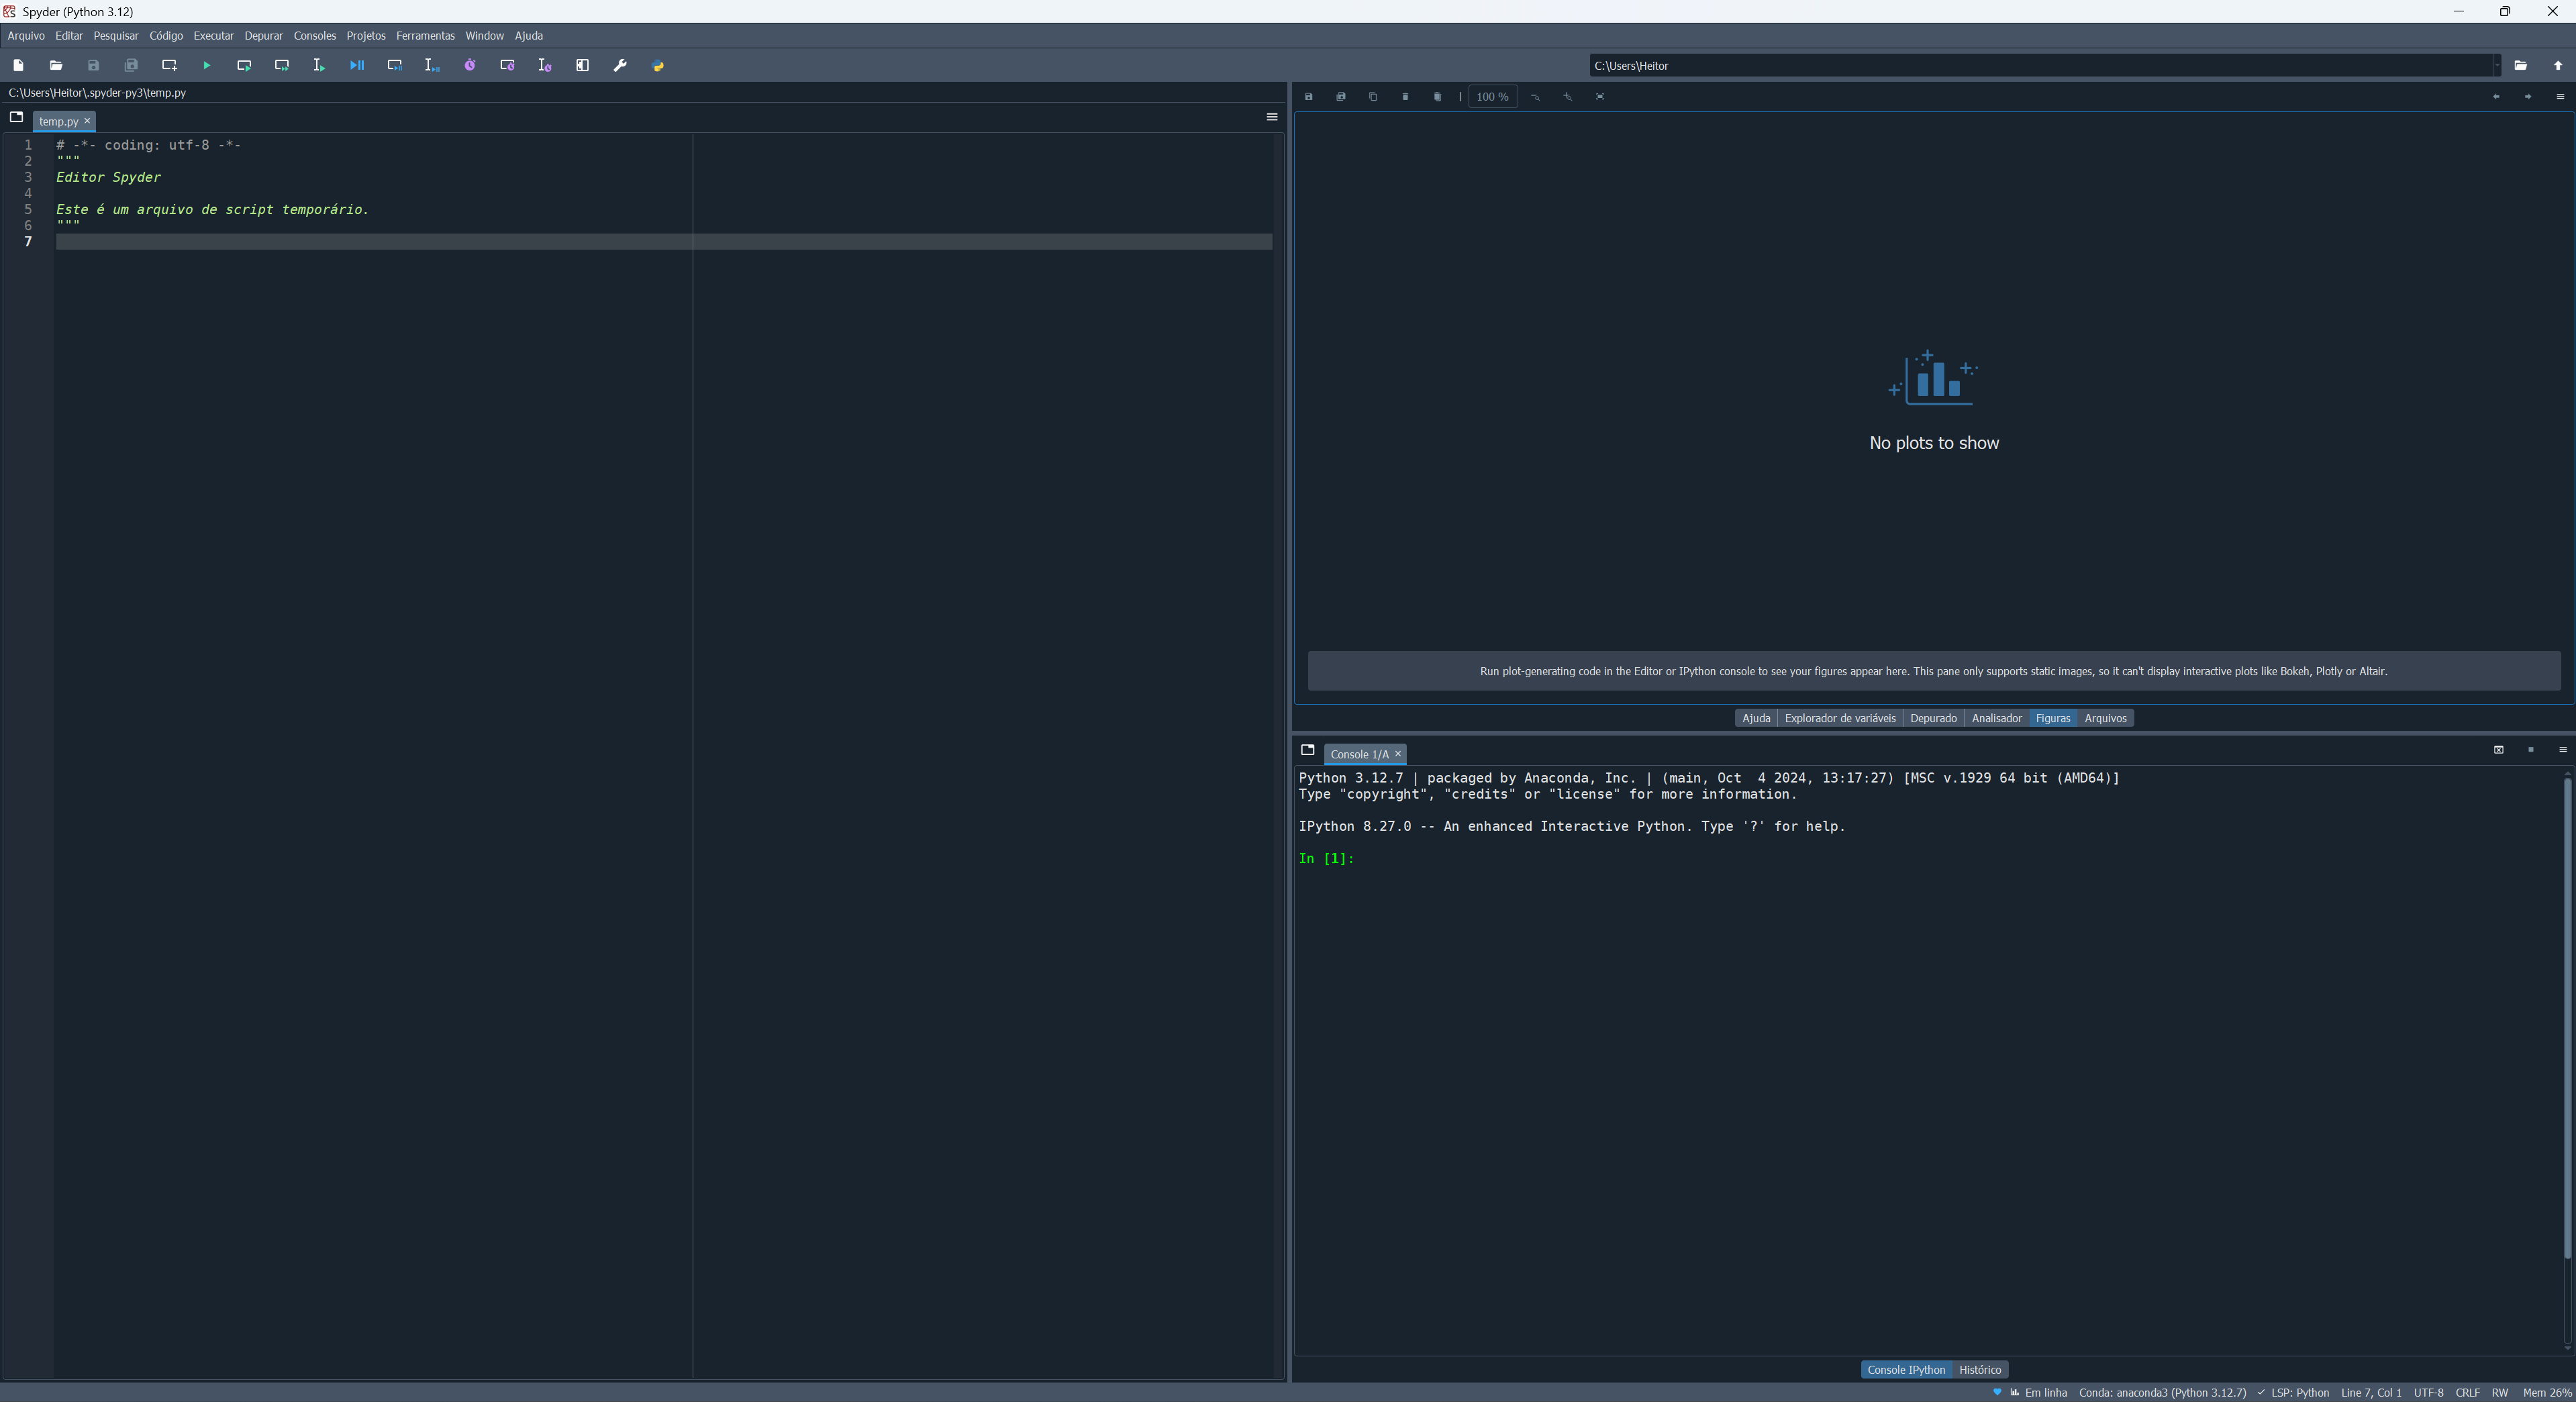
\includegraphics[scale=0.25]{Figures/1-Introducao/Spyder.png}
            \caption{Interface do Spyder ao abri-lo a primeira vez}
            \label{fig:spyder}
        \end{figure}




        Uma recomendação, caso você deseje que as figuras abram em outra janela, é abrir ``Preferências'' (O ícone de chave de boca), ``Console IPython'', ``Plotting'' e mudar ``Saída'' de ``Em linha'' para ``Automático''.
        

        
    \subsection{Revisão programação em Python}

        O Python é uma linguagem de programação bastante simples. Um programa simples para rodar ``Hello World'' é dado da simples forma:

        \begin{lstlisting}[language=Python]
            print("Hello world")
        \end{lstlisting}


        No Python, a indentação (o espaçamento antes de iniciar o texto em cada linha) é fundamental. Este espaçamento indica a hierarquia das estruturas de programação. Ele que indica onde um \textit{if}, \textit{for}, \textit{while}, ou função começa e termina. Por exemplo, o programa a seguir utiliza um \textit{if} para imprimir se um número é par ou ímpar:

        \begin{lstlisting}[language=Python]
            # Em Python, o simbolo # indica um comentario
            N = 3 #Numero inteiro que sera avaliado 
            
            # O simbolo % retorna o resto da divisao
            if N % 2 == 0:
                print(f"O numero {N} e par")
            else:
                print(f"O numero {N} e impar")
        \end{lstlisting}

        Perceba que após o \textit{if}, há um espaçamento com Tab, indicando o que está no \textit{if}. Mesma coisa para o \textit{else}.

        O \textit{for} percorre alguma lista ou vetor. A forma mais tradicional de percorrer um \textit{for} em Python é utilizando o \textit{range}. Observe o programa abaixo que calcula o quadrado de alguns números.

        \begin{lstlisting}[language=Python]
            # Exemplo 1 - calculando o quadrado de 0 a 3
            for i in range(4):
                # Em Python, o operador ^ se faz com **
                print(i**2)

            # >> 0
            # >> 1
            # >> 4
            # >> 9

            # Exemplo 2 - calculando o quadrado de 2 a 3
            for i in range(2,4):
                print(i**2)

            # >> 4
            # >> 9

            # Podemos percorrer diretamente os itens de uma lista
            # Exemplo 3 - calculando o quadrado dos itens de uma lista
            lista = [4, 2, 5]
            for i in lista:
                print(i**2)

            # >> 16
            # >> 4
            # >> 25

            # Uma estrutura Python bem comum tambem se trata do enumerate
            # enumerate retorna o indice do elemento na lista e o valor
            # deste elemento
            # Exemplo 4 - mesmo caso, com enumerate

            lista = [4, 2, 5]
            for i,item in enumerate(lista):
                valor = item**2
                print(f"O quadrado do {i}-esimo elemento e: {valor}")

            # >> O quadrado do 0-esimo elemento e: 16
            # >> O quadrado do 1-esimo elemento e: 4
            # >> O quadrado do 2-esimo elemento e: 25

        \end{lstlisting}


        Outra funcionalidade importante é a definição de funções. Podemos definir uma função com a palavra chave ``def'', em algum lugar do nosso código. Por exemplo, observe o programa abaixo que retorna um número elevado ao outro.

        \begin{lstlisting}[language=Python]
            
            # Funcao que retorna a elevado a b
            def quadrado(a,b):
                return a**b

            # Para rodar a funcao, apenas chamamos ela
            valor1 = quadrado(2,4)
            valor2 = quadrado(5,2)

            print(valor1, valor2)
            # >> 16
            # >> 25

        \end{lstlisting}

        Por último, outra funcionalidade que utilizaremos é a definição de classes. Uma classe é um objeto que carrega consigo algumas funções próprias e variáveis. Nas funções da classe, aparece a variável \textit{self}, que se refere ao próprio objeto. Toda classe tem uma função \_\_\textit{init}\_\_(), que é rodada ao criar uma variável do tipo desta classe.
        
        Por exemplo:

        \begin{lstlisting}[language=Python]
            
            # Classe pessoa, que carrega a idade e o nome.
            
            class Pessoa:

                # Construtor da classe
                def __init__(self, nome, idade):
                    self.nome = nome
                    self.idade = idade

                # Funcao que retorna se aquela pessoa 
                # tem idade para votar
                def pode_votar(self):
                    return self.idade >= 16

            lucas = Pessoa("Lucas",15)
            maria = Pessoa("Maria",40)
            
            print(lucas.pode_votar())
            print(lucas.idade)
            print(maria.pode_votar())
            print(maria.nome)

            # >> False
            # >> 15
            # >> True
            # >> "Maria"

        \end{lstlisting}

        Uma funcionalidade importante de classes é a herança. É possível criar uma classe que herde funções de uma classe pai:

        \begin{lstlisting}[language=Python]
            
            # Classe pessoa, que carrega a idade e o nome.

            class Pessoa:
                def __init__(self, nome, idade):
                    self.nome = nome
                    self.idade = idade

                def pode_votar(self):
                    return self.idade >= 16
            
            class Estudante(Pessoa):

                def __init__(self, nome, idade, curso):
                    #Roda o __init__ da classe pai
                    super().__init__(nome,idade) 
                    self.curso = curso
                
                def nome_do_curso():
                    return self.curso

            leo = Estudante("Leonardo",19,"Engenharia Mecanica")
            maria = Pessoa("Maria",40)
            
            print(leo.pode_votar())
            print(leo.nome_do_curso())
            print(maria.pode_votar())

            # print(maria.nome_do_curso())
            # Nao roda, pois maria e uma Pessoa
            # mas nao e Estudante

            # >> True
            # >> "Engenharia Mecanica"
            # >> True

        \end{lstlisting}
        
        \subsubsection*{Biblioteca Numpy}

        No Python, é usual utilizar bibliotecas que possuem já possuem funções prontas. A biblioteca mais comum para manipulações matemáticas é o Numpy. O Numpy é usado para manipulação de vetores de matrizes, assim como para utilizar funções matemáticas mais comuns. O exemplo abaixo mostra como importar o numpy (usualmente importado sob o nome ``np''), usá-lo para criar um vetor com N pontos linearmente espaçados e calcular o seno desses pontos:

        \begin{lstlisting}
            # Importa biblioteca numpy
            import numpy as np

            # Cria um vetor com 11 pontos linearmente espacados
            # entre 0 e 1, incluindo 0 e 1.
            v = np.linspace(0,1,11)
            print(v)

            # >> [0, 0.1, 0.2, 0.3, 0.4, 0.5, 0.6, 0.7, 0.8, 0.9, 1.0]

            # Calcula o seno dos pontos (v em radianos)
            sen_v = np.sin(v)
            print(sen_v)

            # >>[0.         0.09983342 0.19866933 0.29552021 0.38941834 
            # >> 0.47942554 0.56464247 0.64421769 0.71735609 0.78332691 
            # >> 0.84147098]

        \end{lstlisting}

        Recomenda-se fazer manipulações matemáticas diretamente em um vetor numpy do que fazer termo a termo. Como o Python é uma linguagem interpretada, e o numpy possui funções pré-compiladas, manipular os vetores diretamente é muito mais rápido:

        \begin{lstlisting}
            import numpy as np

            v = np.linspace(0,1,11)

            # Opcao 1 - Lento
            sen_v = np.empty(11) # Cria um vetor tamanho 11 "vazio"
            for i,vi in enumerate(v):
                sen_v[i] = np.sin(vi)

            # Opcao 2 - Mais rapido (recomendado)
            sen_v = np.sin(v)

        \end{lstlisting}

    \subsection{Revisão de conceitos de cálculo}

        Na definição do Método de Elementos Finitos, são necessários alguns conceitos de cálculo. Nesta seção, será apresentado alguns conceitos de cálculo importantes.

        \subsubsection*{Derivada de uma função}

        Seja uma função $f(x)$, sua derivada em um ponto $x=a$ é definida pelo limite:

        \begin{equation*}
            \left.\frac{df}{dx}\right|_{x=a} = f'(a) = \lim_{\Delta x\rightarrow 0 }\frac{f(a+\Delta x)-f(a)}{\Delta x}
        \end{equation*}

        De forma geral, podemos escrever uma função $\frac{df}{dx}$ das derivadas de $f(x)$ em um dado intervalo $\Omega$. As funções mais comuns e suas derivadas são:

        \begin{equation*}
            f(x) = x^n \rightarrow f'(x) = n x^{n-1}
        \end{equation*}

        \begin{equation*}
            f(x) = sen(x) \rightarrow f'(x) = cos(x)
        \end{equation*}

        \begin{equation*}
            f(x) = cos(x) \rightarrow f'(x) = -sen(x)
        \end{equation*}

        E algumas relações importantes são: a \textbf{regra do produto}:

        \begin{equation*}
            \frac{d}{dx}\left(f(x) \cdot h(x)\right) = \frac{df(x)}{dx} \cdot h(x) + f(x) \cdot \frac{dh(x)}{dx},
        \end{equation*}

        \noindent a \textbf{regra do quociente}:

        \begin{equation*}
            \frac{d}{dx}\left(\frac{f(x)}{ h(x)}\right) = \frac{\frac{df(x)}{dx} \cdot h(x) - f(x) \cdot \frac{dh(x)}{dx}}{h(x)^2},
        \end{equation*}

        \noindent e a \textbf{regra da cadeia}:

        \begin{equation*}
            \frac{d}{dx}\left[f(h(x))\right] = \frac{df}{dh} \cdot \frac{dh}{dx},
        \end{equation*}

        A derivada da função derivada é a \textbf{derivada segunda}, e assim sucessivamente:

        \begin{equation*}
            f''(x) = \frac{d^2f}{dx^2} = \frac{df'}{dx}
        \end{equation*}

        \begin{equation*}
            \frac{d^nf}{dx^n} = \frac{d}{dx} \left(\frac{d^{n-1}f}{dx^{n-1}}\right)
        \end{equation*}

        Para funções com mais de uma variável, como $f(x,y,z)$, podemos definir derivadas em relação a cada variável, neste caso, temos uma \textbf{derivada parcial}:

        \begin{equation*}
            \frac{\partial f}{\partial x}, \quad \frac{\partial f}{\partial y}, \quad \frac{\partial f}{\partial z}
        \end{equation*}

        O \textbf{gradiente} de uma função de mais de uma variável é um vetor tal que cada componente é uma derivada parcial:

        \begin{equation*}
            grad \; f = \nabla f = 
            \begin{Bmatrix}
                \frac{\partial f}{\partial x}\\
                \frac{\partial f}{\partial y}\\
                \frac{\partial f}{\partial z}
            \end{Bmatrix}
        \end{equation*}

        Uma \textbf{função vetorial}, é um vetor que cada termo é uma função, por exemplo:

        \begin{equation*}
            \mathbf{f}(x,y) = 
            \begin{Bmatrix}
                f_1(x,y)\\
                f_2(x,y)
            \end{Bmatrix}
        \end{equation*}

        O \textbf{divergente} de uma função vetorial é a soma das derivadas em relação a cada variável:

        \begin{equation*}
            div \; \mathbf{f} = 
            \nabla \cdot \mathbf{f} = 
            \frac{\partial f_1}{\partial x} + \frac{\partial f_2}{\partial y}
        \end{equation*}

        O gradiente de uma função vetorial é uma matriz em que cada linha é o gradiente de cada função

        \begin{equation*}
            grad \; \mathbf{f} = 
            \nabla \mathbf{f} = 
            \begin{bmatrix}
                \frac{\partial f_1}{\partial x} & \frac{\partial f_2}{\partial x} \\
                \frac{\partial f_1}{\partial y} & \frac{\partial f_2}{\partial y}
            \end{bmatrix}
        \end{equation*}

        O \textbf{laplaciano} é o divergente do gradiente de uma função escalar:

        \begin{equation*}
            \Delta f(x) = \nabla \cdot \left(\nabla f(x)\right) = \nabla \cdot 
            \begin{Bmatrix}
                \frac{\partial f}{\partial x}\\
                \frac{\partial f}{\partial y}
            \end{Bmatrix} =
            \frac{\partial^2 f_1}{\partial x^2} + \frac{\partial^2 f_2}{\partial y^2}
        \end{equation*}


        \subsubsection*{Integral de uma função}

        Nesta disciplina, usaremos integrais definidas. Uma integral definida (integral de Riemann) em um intervalo $\Omega = (a,b)$ é definida como:
        
        \begin{equation*}
            \int_{a}^{b} f(x) dx = \lim_{i\rightarrow\infty} \sum_{i=1}^n f(x_i) \Delta x_i, \quad \Delta x_i = \frac{b-a}{n}
        \end{equation*}

        Segundo o teorema fundamental do cálculo, uma integral pode ser vista como a operação inversa da derivada:

        \begin{equation}
            \int_{a}^{b} f'(x) dx = f(b)-f(a)
        \end{equation}

        Portanto, para integrar uma função, normalmente utilizam-se procedimentos para facilitar encontrar a função cuja derivada é o integrando. 
        
        Um procedimento é o da \textbf{substituição de variáveis}. Dada a integral:

        \begin{equation*}
            \int_{x_1}^{x_2} f(x) dx
        \end{equation*}
        
        \noindent se conseguirmos definir uma variável $y$, com $x(y)$, tal que $dx = \frac{dx}{dy} dy$, $x_1 = x(y_1)$ e $x_2 = x(y_2)$. Então podemos reescrever a integral como:

        \begin{equation*}
            \int_{x_1}^{x_2} f(x) dx = 
            \int_{y_1}^{y_2} f(x(y)) \frac{dx}{dy} dy
        \end{equation*}
        
        Outro procedimento usual é a \textbf{integração por partes:}

        \begin{equation}
            \int_{a}^{b} f'(x) h(x) dx = \left[f(x)h(x)\right]_{a}^{b} - \int_{a}^{b} f(x) h'(x) dx
        \end{equation}


        Uma integral dupla, tripla, e assim sucessivamente, é uma integral definida de funções de mais de uma variável:

        \begin{equation*}
            \int_{y_1}^{y_2} \int_{x_1}^{x_2} f(x,y) dx dy
        \end{equation*}

        Em uma área qualquer $\Omega$, vamos escrever como:

        \begin{equation*}
            \int_{\Omega} f(x,y) dA
        \end{equation*}

        Considerando uma área $\Omega$ definida pelo sistema de coordenadas $xy$, podemos realizar uma mudança de coordenadas na integração para a mesma área, porém descrita por um sistema de coordenadas diferente $\hat{x}\hat{y}$, da seguinte forma:

        \begin{equation*}
            \int_{\Omega} f(x,y) dA = \int_{\Omega} f(x(\hat{x},\hat{y}),y(\hat{x},\hat{y})) \det \mathbf{J} d\hat{A}
        \end{equation*}

        \noindent no qual:

        \begin{equation*}
            \mathbf{J} = 
            \begin{bmatrix}
                \frac{\partial x}{\partial \hat{x}} & \frac{\partial y}{\partial \hat{x}}\\
                \frac{\partial x}{\partial \hat{y}} & \frac{\partial y}{\partial \hat{y}}
            \end{bmatrix}
        \end{equation*}

        Dada uma superfície $\Gamma$ no espaço $\mathbb{R}^3$, uma \textbf{integral de superfície} é dada por:

        \begin{equation*}
            \int_{\Gamma} f dS
        \end{equation*}

        O \textbf{teorema do divergente} transforma a integral no volume do divergente de uma função vetorial em uma integral de superfície, ao longo da superfície do domínio de integração original:

        \begin{equation*}
            \int_{\Omega} \nabla \cdot \mathbf{f} dV = \int_{\partial \Omega}  \mathbf{f} \cdot \mathbf{n} dS
        \end{equation*}

        \noindent no qual $\partial \Omega$ é o fecho de $\Omega$, isto é, o contorno fechado de $\Omega$, e $\mathbf{n}$ é o vetor normal à superfície, apontando para fora.

    \subsection{Revisão de conceitos de álgebra linear}
    \label{sec:algelin}

        A álgebra linear, embora não estritamente necessária para ter um entendimento básico e para aplicar o Método dos Elementos Finitos, é essencial para entender mais a fundo como este funciona. Portanto, esta seção apresenta a revisão de alguns conceitos básicos de espaço vetorial, e apresenta alguns espaços citados no texto.

        Um corpo $K$ é um conjunto no qual as operações de adição e multiplicação entre termos são definidas e satisfazem as seguintes condições:

        Axiomas da adição:
        \begin{itemize}
            \item \textit{Associatividade:} $(a+b)+c = a+(b+c)$
            \item \textit{Comutatividade:} $a+b=b+a$
            \item \textit{Elemento neutro:} $\exists 0 \in K : a+0=a, \forall a \in K$
            \item \textit{Simétrico:} $\forall a \in K, \exists (-a)\in K : a + (-a) = 0$
        \end{itemize}

        Axiomas da multiplicação:
        \begin{itemize}
            \item \textit{Associatividade:} $(a \cdot b) \cdot c = a \cdot (b \cdot c)$
            \item \textit{Comutatividade:} $a \cdot b=b \cdot a$
            \item \textit{Elemento neutro:} $\exists 1 \in K, 1\neq 0 : a \cdot 0 = 0, \forall a \in K$
            \item \textit{Inverso multiplicativo:} $\forall a \neq 0 \in K : \exists a^{-1}\in K : a \cdot a^{-1} = 1$
        \end{itemize}

        Um corpo ordenado é aquele no qual os seus elementos podem ser descritos como positivos, negativos ou zero. O conjunto dos números reais $\mathbb{R}$ é um corpo ordenado completo.

        Um espaço vetorial $V$ sobre um corpo $K$ é um conjunto munido das operações de soma entre dois elementos de $V$ e de multiplicação por escalar, entre um elemento de $K$ e um elemento de $V$. Estas operações devem obedecem aos seguintes axiomas:

        \begin{itemize}
            \item \textit{Associatividade da adição:} $(\mathbf{u} + \mathbf{v}) + \mathbf{w} = \mathbf{u} + (\mathbf{v} + \mathbf{w})$
            \item \textit{Comutatividade da adição:} $\mathbf{u} + \mathbf{v} = \mathbf{v} + \mathbf{u}$
            \item \textit{Elemento neutro na adição:} $\exists \mathbf{0} \in V :\mathbf{u} + \mathbf{0} = \mathbf{u}$
            \item \textit{Simétrico na adição:} $\forall \mathbf{u} \in V, \exists (\mathbf{-u}) \in V :\mathbf{u} + (\mathbf{-u}) = \mathbf{0}$
            \item \textit{Associatividade na multiplicação por escalar:} $a,b \in K, u \in V : a(b\mathbf{u}) = (ab)\mathbf{u}$
            \item \textit{Elemento neutro na multiplicação por escalar:} seja $1$ o elemento neutro de $K : 1\mathbf{u} = \mathbf{u}$
            \item \textit{Distributividade do vetor na multiplicação por escalar:} $a(\mathbf{u} + \mathbf{v}) = a\mathbf{u} + a\mathbf{v}$
            \item \textit{Distributividade do escalar na multiplicação por escalar:} $(a+b)\mathbf{u} = a\mathbf{u} + b\mathbf{u}$
        \end{itemize}

        O espaço vetorial mais fácil de entender visualmente é o espaço vetorial dos vetores em $\mathbb{R}^3$, representado por ``setas'' no espaço tridimensional. Entretanto, essas definições podem ser aplicadas mesmo em conceitos mais amplos de espaço vetorial.

        A \textbf{dimensão} de um espaço vetorial é número de variáveis independentes (em $K$) necessárias e suficientes para representar, de forma única, um vetor em $V$. Por exemplo, o espaço $\mathbb{R}^3$ tem dimensão $3$, pois precisamos de três números independentes para representar um vetor, por exemplo, suas três componentes no sistema cartesiano.

        Uma \textbf{base} é um conjunto de vetores linearmente independentes que podem representar qualquer vetor do espaço vetorial. Um conjunto de vetores linearmente independentes de um espaço de dimensão $n$ ($\mathbf{u}_1, \mathbf{u}_2, \ldots, \mathbf{u}_n$) é aquele que nenhum vetor da base pode ser escrito como uma combinação linear dos outros, isto é, não existe nenhuma combinação de escalares ($a_1, a_2, \ldots, a_n$), tal que um vetor possa ser escrito como uma soma dos outros:

        \begin{equation}
            \mathbf{u}_j \neq a_1 \mathbf{u}_1 + \cdots + a_{j-1} \mathbf{u}_{j-1} + a_{j+1} \mathbf{u}_{j+1} + \cdots + a_n \mathbf{u}_n = \sum\limits_{\underset{i\neq j}{i=0}}^n a_i \mathbf{u}_i , \quad \forall a_1, a_2, \ldots, a_n \in K
        \end{equation}

        Qualquer vetor do espaço vetorial pode ser escrito de forma única como uma combinação linear dos vetores que formam uma base:

        \begin{equation}
            \mathbf{v} = a_1 \mathbf{u}_1 + \cdots + a_{i} \mathbf{u}_{i} + \cdots + a_n \mathbf{u}_n = \sum\limits_{i=0}^n a_i \mathbf{u}_i
        \end{equation}

        Por exemplo, para o espaço vetorial $\mathbb{R}^3$, normalmente é usada a base ortogonal dos vetores unitários $\mathbf{i}, \mathbf{j}, \mathbf{k}$, de forma que qualquer $\mathbf{u}$ pode ser escrito como:

        \begin{equation}
            \mathbf{u} = u_x \mathbf{i} + u_y \mathbf{j} + u_z \mathbf{k}
        \end{equation}

        O espaço vetorial dos polinômios de grau menor ou igual a $2$, denominado $\mathcal{P}_2$, tem dimensão $3$ e pode ser escrito pela base $p_1(x) = 1, p_2(x) = x, p_3(x) = x^2$, tal que, para qualquer polinômio deste espaço:

        \begin{equation}
            q(x) = a_0 + a_1x + a_2 x^2 = a_0 p_1(x) + a_1 p_2(x) + a_2 p_3(x)
        \end{equation}
    
        Existem espaços vetoriais de \textbf{dimensão infinita}, isso significa que não é possível escrever uma base para este espaço. Um exemplo de espaço vetorial de dimensão infinita é o espaço formado pelas funções suaves (funções contínuas com todas as derivadas contínuas) $\mathcal{C}^\infty$.

        Um \textbf{subespaço} é um espaço vetorial que é subconjunto de um espaço vetorial. Por exemplo, o espaço vetorial dos polinômios de grau menor ou igual 2 $\mathcal{P}_2$ é composta por funções suaves, portanto, $\mathcal{P}_2$ é um subespaço de $C^\infty$. Da mesma forma, polinômios de grau menor ou igual a 2 têm grau menor ou igual a 5, então $\mathcal{P}_2$ é um subespaço de $\mathcal{P}_5$. Note que subespaços sempre devem ter dimensão menor ou igual à dimensão do espaço maior.

        O \textbf{produto interno} é uma operação $\left\langle \cdot, \cdot \right\rangle $ entre dois vetores de um espaço vetorial que retornam um escalar. Ele deve obedecer às relações:

        \begin{itemize}
            \item \textit{Simetria conjugada:} $\left\langle \mathbf{u}, \mathbf{v} \right\rangle = \bar{\left\langle \mathbf{v}, \mathbf{u} \right\rangle}$
            \item \textit{Linearidade:} $\left\langle a\mathbf{u} + b\mathbf{v}, \mathbf{w} \right\rangle = \left\langle a\mathbf{u}, \mathbf{w} \right\rangle + \left\langle b\mathbf{v}, \mathbf{w} \right\rangle$
            \item \textit{Positividade:} $\left\langle \mathbf{u}, \mathbf{u} \right\rangle > 0 , \quad\forall \mathbf{u} \neq \mathbf{0}$
        \end{itemize}

        O exemplo mais usual de produto interno é o produto escalar entre vetores euclideanos:

        \begin{equation}
        \left\langle \mathbf{u}, \mathbf{v} \right\rangle  = 
        \mathbf{u} \cdot \mathbf{v} =
        \begin{Bmatrix}
            u_1\\
            u_2\\
            \vdots\\
            u_n
        \end{Bmatrix} \cdot
        \begin{Bmatrix}
            v_1\\
            v_2\\
            \vdots\\
            v_n
        \end{Bmatrix}
        =
        u_1 v_1 + u_2 v_2 + \cdots + u_n v_n
    \end{equation}

    Em espaços definidos por funções, o produto interno mais comum é dado por uma integral definida:

    \begin{equation}
        \left\langle p(x), q(x) \right\rangle  = \int_{a}^{b} p(x) \bar{q(x)} dx
    \end{equation}

    Dois vetores são ditos \textbf{ortogonais} se o produto interno entre eles for nulo. Desta forma, uma base ortogonal é formada por vetores linearmente independentes que também são ortogonais entre si.

    A definição de \textbf{norma} é baseada no produto interno e presenta uma operação do vetor sobre ele mesmo que retorna um escalar. Por exemplo, no espaço euclideano:

    \begin{equation}
        \left\Vert \mathbf{u} \right\Vert = \sqrt{\left\langle \mathbf{u},\mathbf{u} \right\rangle} = \sqrt{ u_1^2 + u_2^2 + \cdots + u_n^2}
    \end{equation}

    No caso de funções com o produto interno definido pela integral:

    \begin{equation}
        \left\Vert p(x) \right\Vert = \sqrt{\left\langle p(x),p(x) \right\rangle} = \int_{a}^{b} p(x)^2 dx
    \end{equation}

    \noindent como veremos logo a seguir, na próxima seção, o espaço vetorial munido dessa operação é chamado espaço de Lebesgue.

    \subsubsection*{Espaço de Sobolev}

    Com as definições anteriores, definiremos alguns espaços vetoriais de funções. O espaço $\mathcal{C}^p (\Omega)$ (às vezes representado apenas por $\mathcal{C}^p$) já citado anteriormente, é o espaço composto pelas contínuas em $\Omega$ e com até a $p$-ésima derivada também contínua em $\Omega$. Por exemplo, a função rampa:

        \begin{equation*}
            f(x) = \left\{\begin{array}{l}
                x, x \geq 0\\
                0, x<0
            \end{array}\right.,
        \end{equation*}

    é contínua, mas possui derivada não contínua no intervalo $\Omega = ]-\infty, \infty[$, portanto $f(x) \in \mathcal{C}^0(\Omega)$. Porém, no intervalo $\Omega_2 = [3, 10]$, por exemplo, ele possui derivadas contínuas não importa a ordem (a partir da segunda, se anula). Portanto, $f(x) \in \mathcal{C}^\infty(\Omega)$. O espaço $\mathcal{C}^\infty$ muitas vezes é chamado de espaço das \textbf{funções suaves}.


    Com as definições anteriores, podemos definir o \textbf{espaço de Lebesgue} $\mathcal{L}^p(\Omega)$. Este é composto pela funções $p$-integráveis, isto é:

        \begin{equation}
            \int_\Omega \left|f(x)\right|^p dx < \infty
        \end{equation}

    Normalmente, definem-se as funções quadrado integráveis $\mathcal{L}^2(\Omega)$:

    \begin{equation}
        \int_\Omega \left[f(x)\right]^2 dx < \infty
    \end{equation}

    A importância deste espaço, é que este define um espaço com um produto interno finito para todos os membros deste espaço, isto é:

    \begin{equation}
        \left\langle f(x), h(x) \right\rangle = \int_\Omega f(x)h(x) dx < \infty
    \end{equation}

    Finalmente, temos o \textbf{espaço de Sobolev} $\mathcal{H}^p(\Omega)$. Um espaço de Sobolev de ordem $p$ é aquele que todas as funções e todas as suas respectivas derivadas até a ordem $p$ pertencem a $\mathcal{L}^2(\Omega)$. Isto é:

    \begin{equation}
        \int_\Omega \left[f(x)\right]^2 dx < \infty
    \end{equation}

    \begin{equation}
        \int_\Omega \left[\frac{d^nf}{dx^n}\right]^2 dx < \infty \quad, \forall n \leq p
    \end{equation}

    A importância deste tipo de espaço está na solução de equações diferenciais. Considere a equação diferencial de ordem $n$ abaixo em algum domínio $\Omega$:

    \begin{equation*}
        p\left(x, f(x), \frac{df}{dx}, \ldots, \frac{d^nf}{dx^n}\right) + q(x) = 0,
    \end{equation*}

    \noindent então sabemos que, se existir solução, ela será um membro de $\mathcal{H}^p(\Omega)$.

    Esta relação será utilizada nos métodos para obter soluções aproximadas de equações diferenciais mostrados aqui. A solução da equação pertence ao espaço vetorial de dimensão infinita $\mathcal{H}^p(\Omega)$. A aproximação se baseará em encontrar a função em um subespaço de $\mathcal{H}^p(\Omega)$ de dimensão finita, por exemplo $\mathcal{P}_q$, que melhor se aproxima da solução real.